\paragraph{}El usuario administrador principal puede realizar consultas sobre
los centros, departamentos, titulaciones, asignaturas, asesores, alumnos y sobre
las plantillas oficiales que existan en el sistema.
\textit{Además también puede realizar consultar de datos históricos referentes a
esta misma información en diferentes cursos académicos}.

\paragraph{}La figura \ref{diagramaNivel3-ExplotacionSistema-adminPrincipal}
muestra el nivel de abstracción 3: Explotación del sistema (módulo Administrador
principal).

  \begin{figure}[!ht]
    \begin{center}
      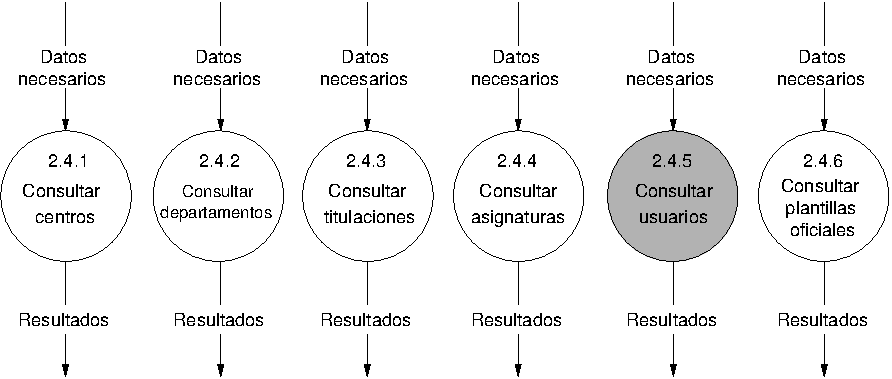
\includegraphics[]{08.Analisis_Funcional/8.2.DFDs/Niveles/Nivel3/AdministradorPrincipal/ExplotacionSistema/Diagramas/nivel3-ExplotacionSistema.pdf}
      \caption{Nivel de abstracción 3: Explotación del sistema (módulo
      Administrador principal).}
      \label{diagramaNivel3-ExplotacionSistema-adminPrincipal}
    \end{center}
  \end{figure}